% Companion figure gallery for the ICTAC 2026 tool paper
% "Tool Support for Causal Reasoning via String Diagram Surgery".
% These diagrams are produced by the tool (Chyp exports) and are referenced
% from the paper and the repository README; they are kept here, outside the
% page-limited submission, for full-resolution inspection.
\documentclass[11pt]{article}
\usepackage[a4paper,margin=2.2cm]{geometry}
\usepackage{graphicx}
\graphicspath{{paper/}}
\usepackage{amsmath}
\usepackage{caption}
\usepackage{hyperref}

\title{Diagram Gallery\\[2pt]
\large Companion to ``Tool Support for Causal Reasoning via String Diagram Surgery''}
\author{Sifei Li and Fabio Zanasi \\ University College London}
\date{}

\begin{document}
\maketitle

\noindent
This companion document collects the full-resolution diagrams produced by the
tool for the running \emph{commute} example, omitted from the page-limited
submission for space. Each figure corresponds to a stage of the pipeline
described in the paper (Section~3); diagrams from Step~2 onward are direct
\textbf{Chyp exports} written to the \texttt{trace/} directory by the tool, so
they show exactly what a user inspects when running the pipeline. (Chyp uses a
limited character set, so some symbols are mangled in the labels.) The raw
\texttt{.chyp} sources are under \texttt{trace/commute/} in the repository.

\bigskip

\begin{figure}[h]
\centering
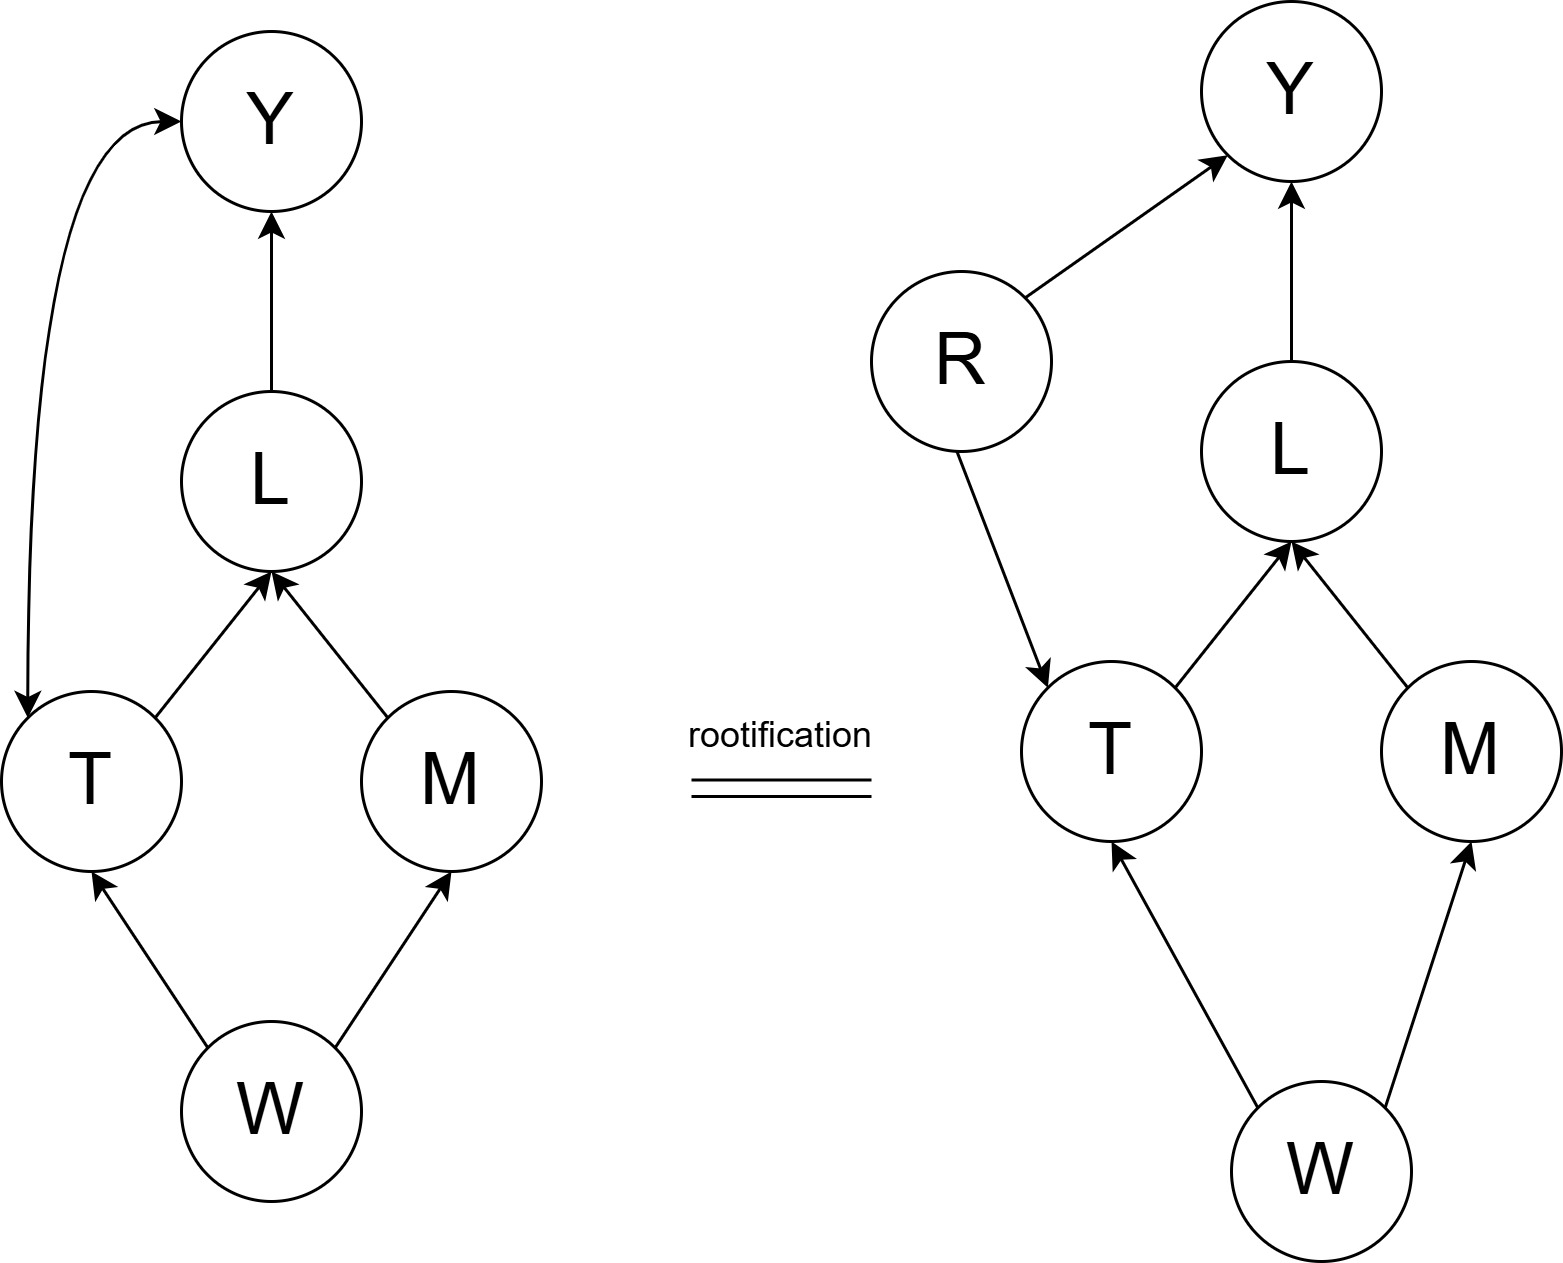
\includegraphics[width=0.92\linewidth,height=0.34\textheight,keepaspectratio]{ADMG.png}
\caption{\textbf{Stage 1 --- ADMG compilation (rootification).} The input
Acyclic Directed Mixed Graph for the commute model (left) and its rootified form
(right), in which the bidirected edge $T\leftrightarrow Y$ is replaced by a fresh
latent root $R$ feeding both $T$ and $Y$.}
\end{figure}

\begin{figure}[h]
\centering
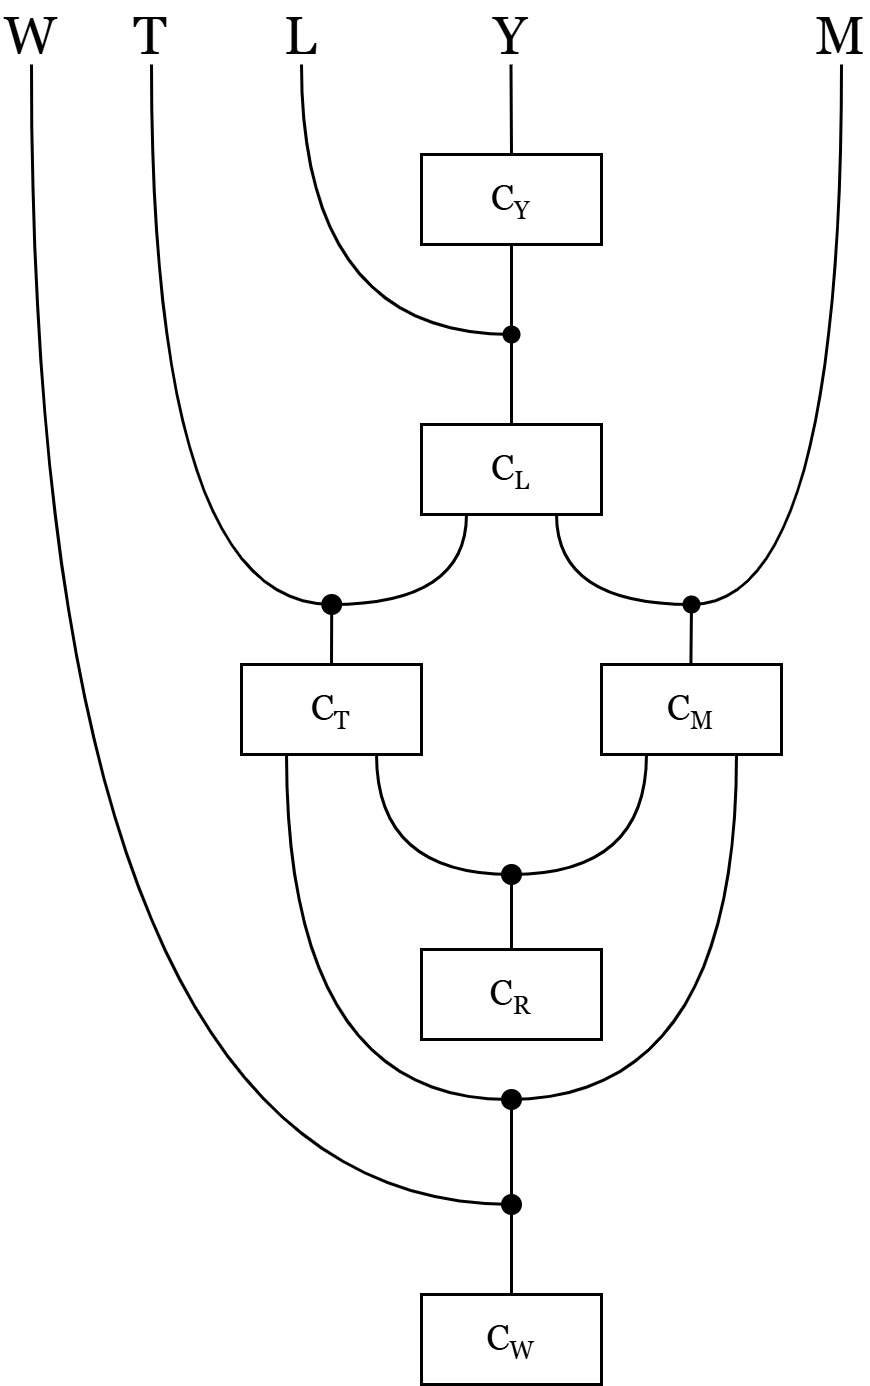
\includegraphics[width=0.48\linewidth,height=0.40\textheight,keepaspectratio]{String_diagram.png}
\hfill
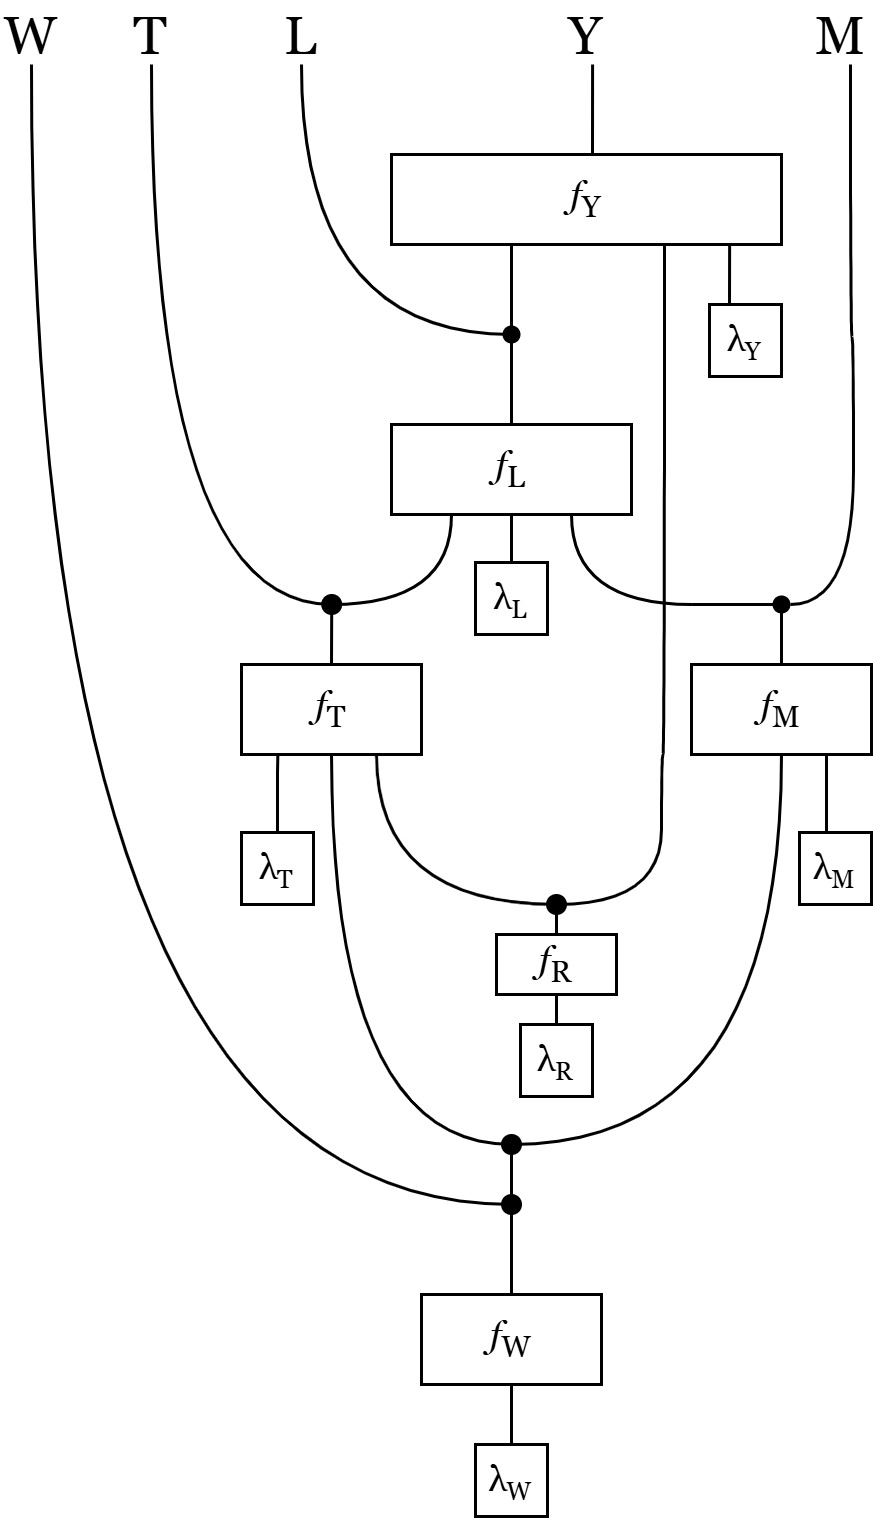
\includegraphics[width=0.48\linewidth,height=0.40\textheight,keepaspectratio]{FCM.jpg}

\caption{\textbf{Stage 1 (cont.) --- compiled string diagram.}
The commute model as a Catlab wiring diagram: each variable becomes a mechanism box,
copy dots duplicate values feeding several mechanisms, and the shared latent root
realises the confounding $T\leftrightarrow Y$.}
\end{figure}

\clearpage

\begin{figure}[h]
\centering
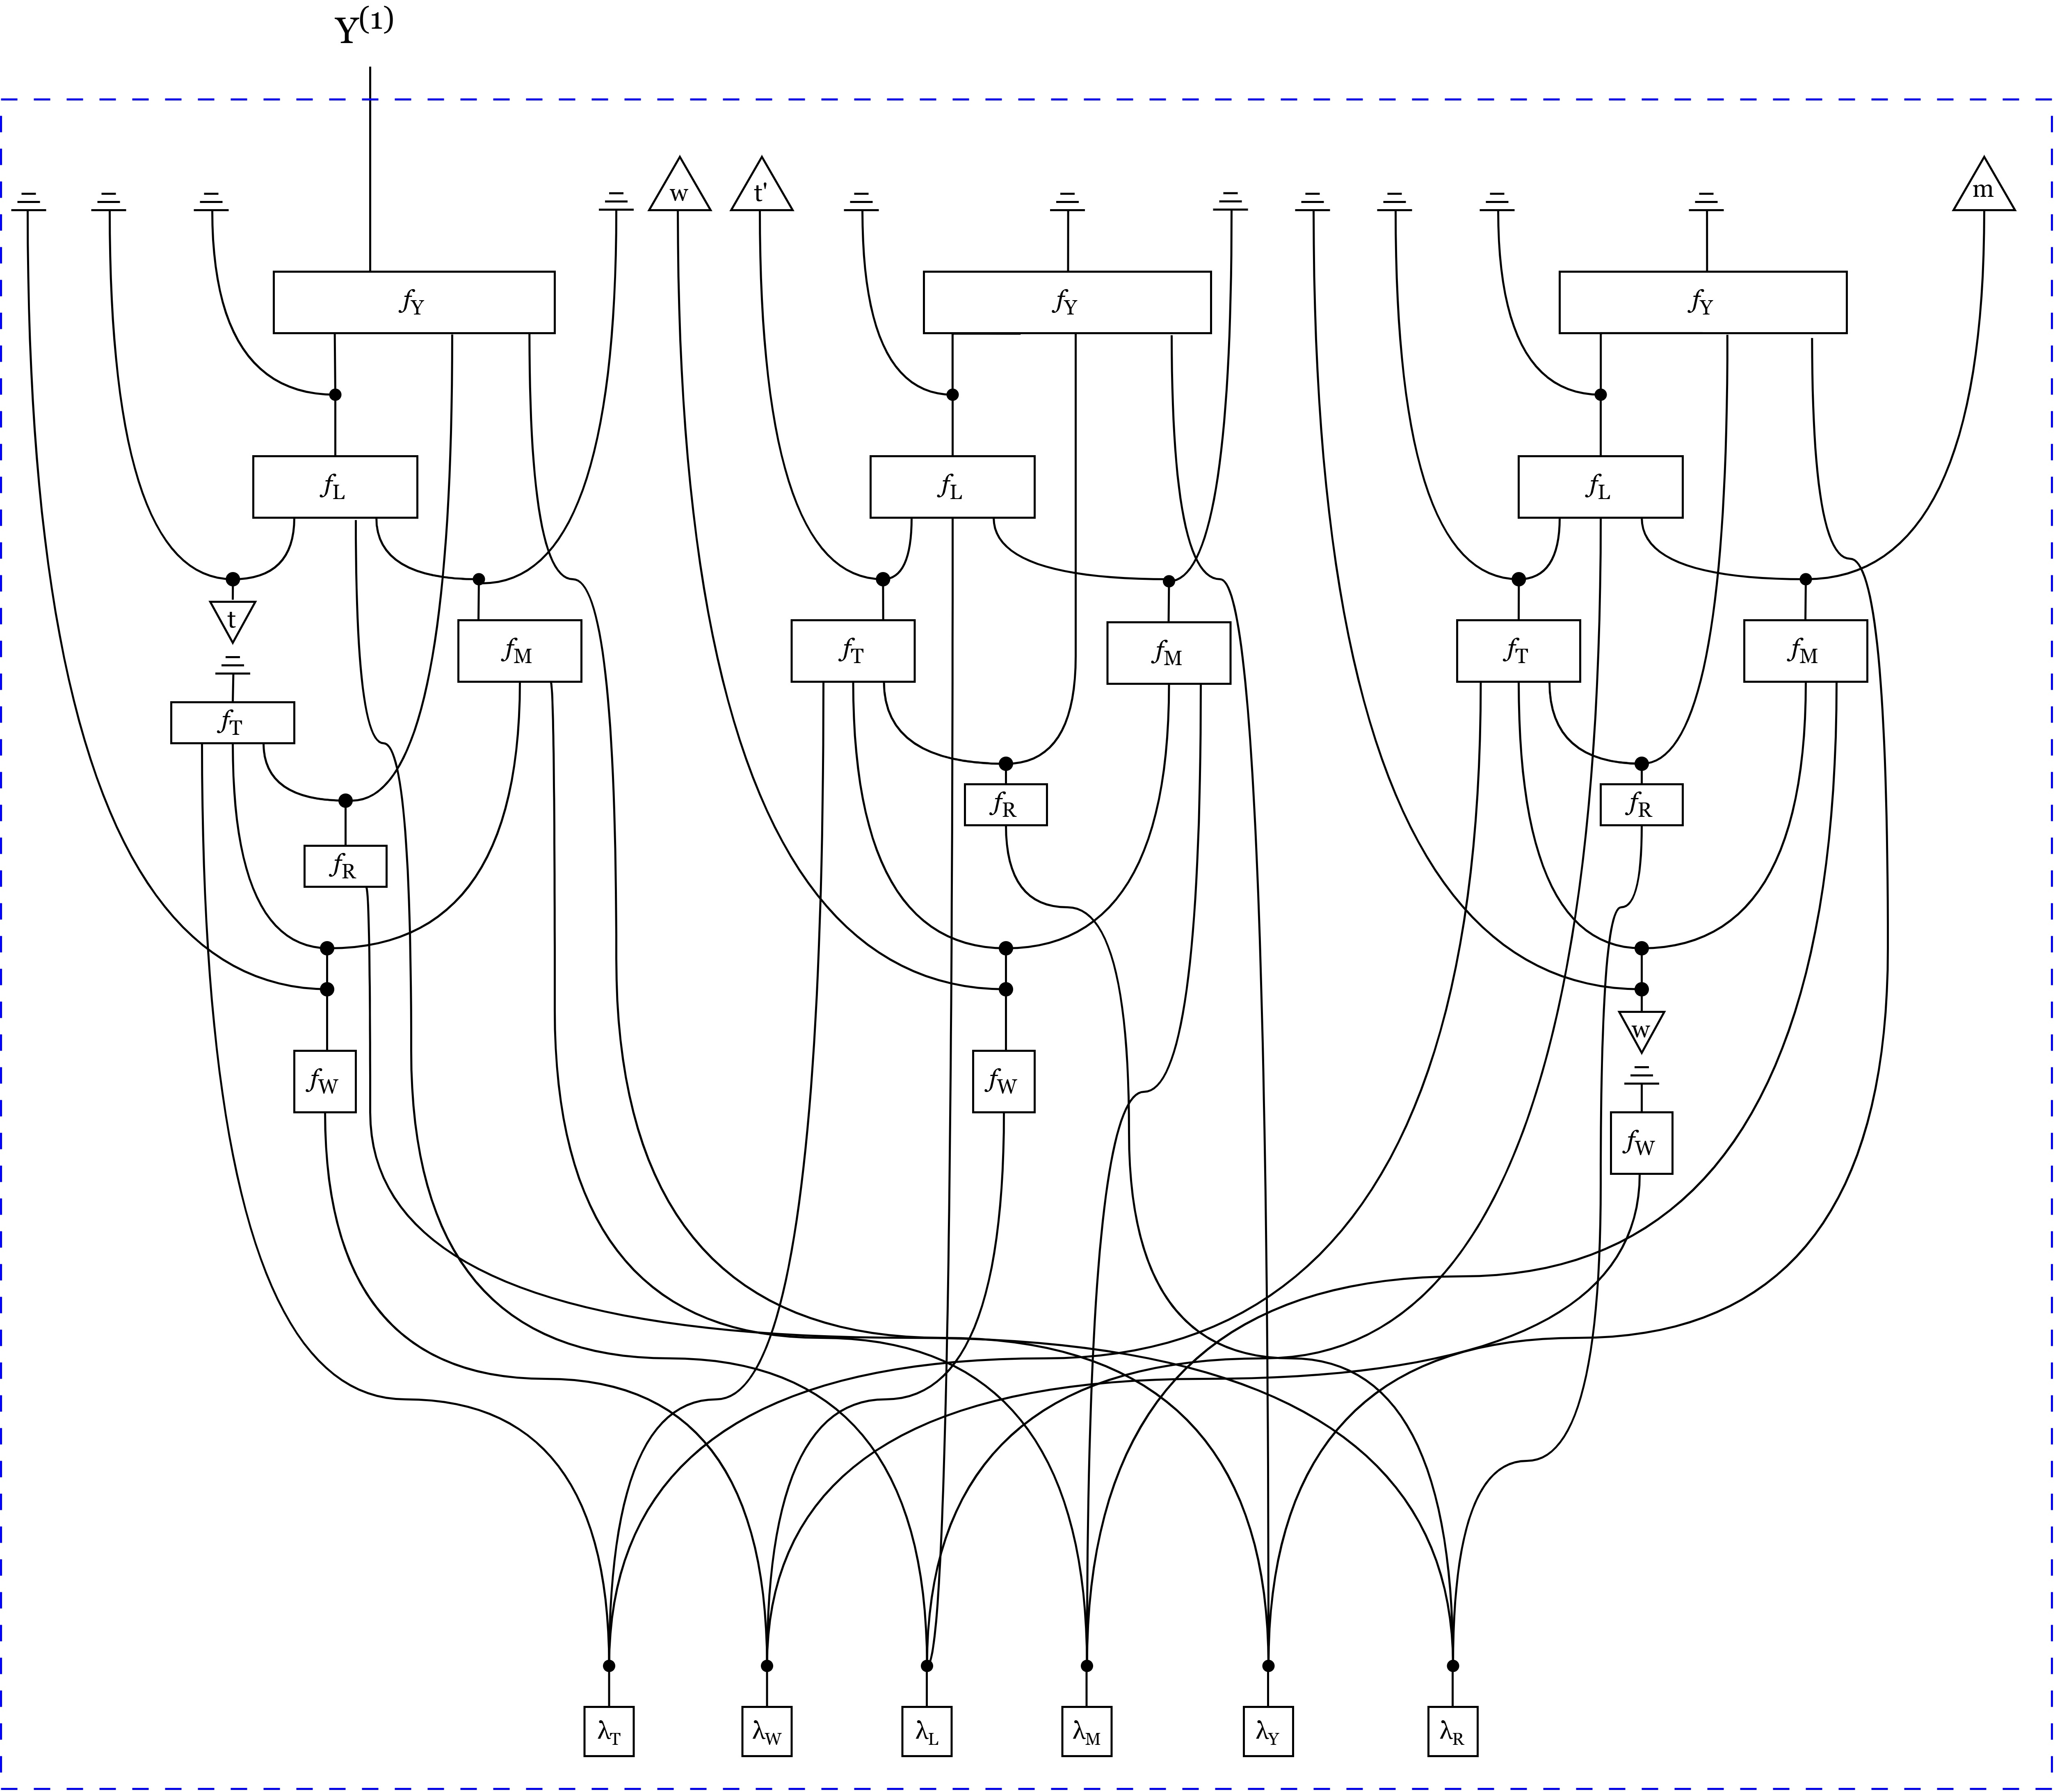
\includegraphics[width=0.95\linewidth,height=0.62\textheight,keepaspectratio]{muti.png}
\caption{\textbf{Stage 2 --- parallel-world (twin) construction.} The base
diagram lifted into a multiverse: each mechanism is duplicated per world while
the exogenous sources are shared, so the factual and counterfactual worlds stay
coupled through the common latent structure. Surgery $\mathrm{do}(T{=}t)$ is
applied only in the counterfactual world.}
\end{figure}

\clearpage

\begin{figure}[h]
\centering
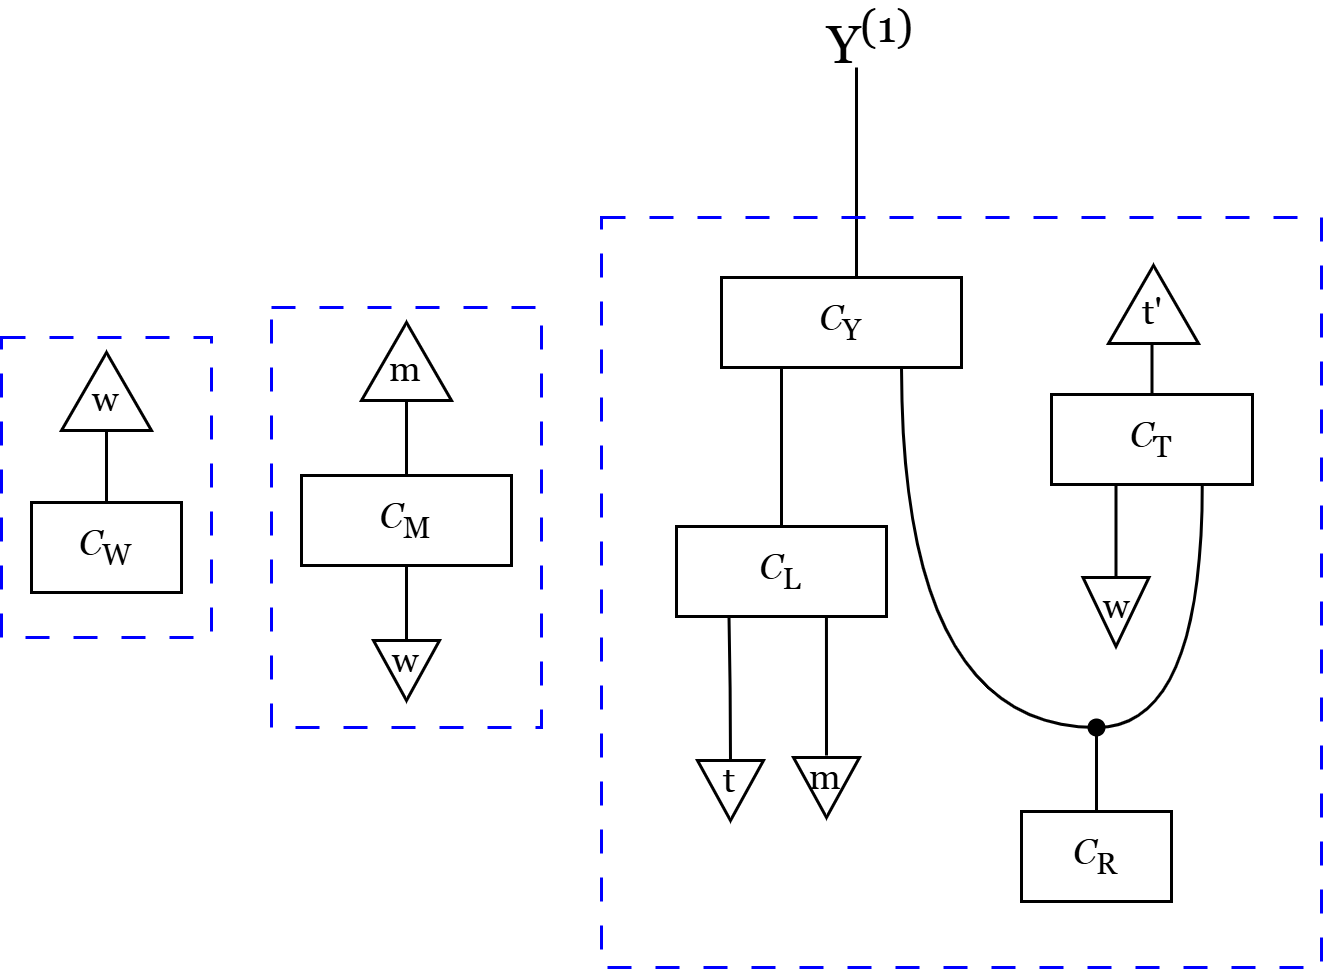
\includegraphics[width=0.95\linewidth,height=0.45\textheight,keepaspectratio]{simplify.png}
\caption{\textbf{Stage 3 --- simplified diagram.} The diagram after the four
rewrite passes (pruning, observation separation, deterministic-mechanism
merging, exogenous-source absorption) reduce it to canonical form.}
\end{figure}

\begin{figure}[h]
\centering
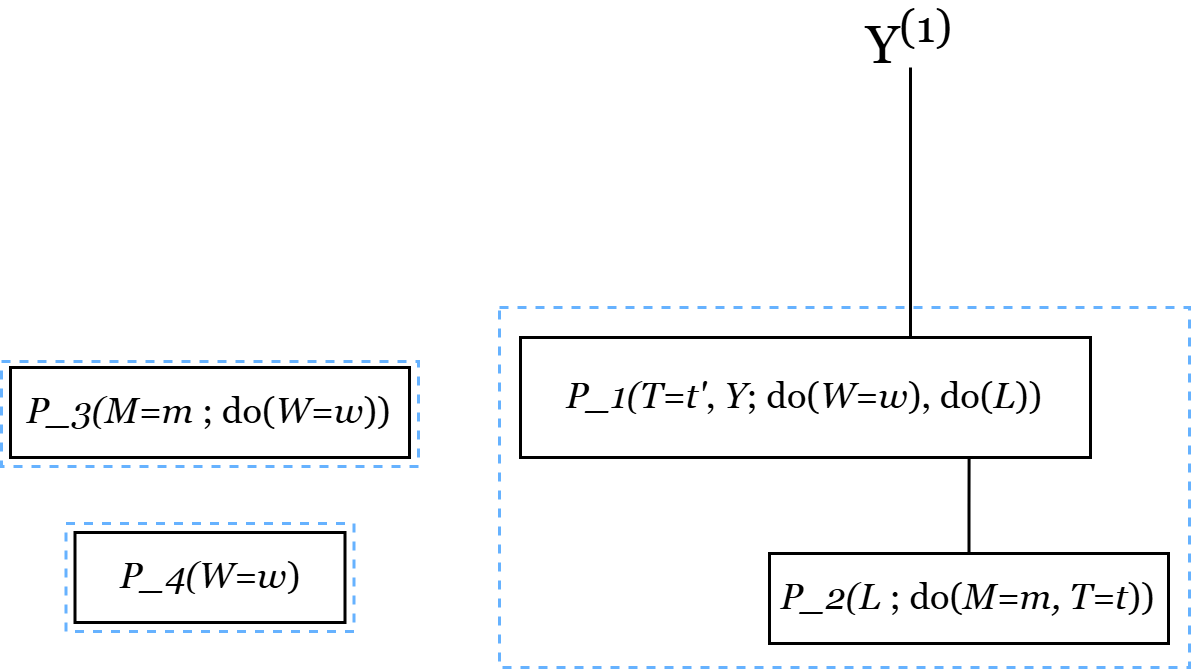
\includegraphics[width=0.95\linewidth,height=0.40\textheight,keepaspectratio]{idcf.png}
\caption{\textbf{Stages 4--5 --- identified estimand.} The R-fragments rewritten
into interventional probability boxes and rendered as the final estimand. A
residual unabsorbed exogenous source would instead signal a non-identifiable
query.}
\end{figure}

\end{document}
